\documentclass{article}

\hyphenchar\font=-1 % suppress hyphenation
\setlength\parindent{0pt} % suppress indentation
\usepackage[margin=1.5truein]{geometry} % set page margins

\usepackage{tikz}
\usetikzlibrary{arrows,automata,positioning}
\usepackage{pgfplots}

\usepackage{fancyhdr}
\usepackage{lastpage}
\usepackage{url}
\usepackage{xcolor}
\usepackage{hyperref}
\usepackage{natbib}

\hypersetup{
    colorlinks = true,
    linkcolor = red,
    urlcolor = red,
    citecolor = black
}

%% page numbering
\pagestyle{fancy}
\fancyhf{}
\fancyfoot[C]{Pg. \thepage \space of \pageref*{LastPage}}
\renewcommand{\headrulewidth}{0pt}

\begin{document}
\title{SYSEN 6000: Foundations of Complex Systems\\~\\
    \Large Causal Loops \& Emergent Behavior
}
\author{
    Nick Kunz [NetID: \url{nhk37}] \hyperlink{nhk37@cornell.edu}{nhk37@cornell.edu}}
\date{September 14, 2022}
\maketitle
\thispagestyle{fancy}

\section*{Casual Loops: Prediction Systems}
The goal of this analysis was to broadly illustrate the causal relationships between system level considerations for the most important theoretical bounds of prediction systems, as they relate to synthetic data in machine learning. It is meant to serve as a basis for future research in that regard.
    \begin{center}
        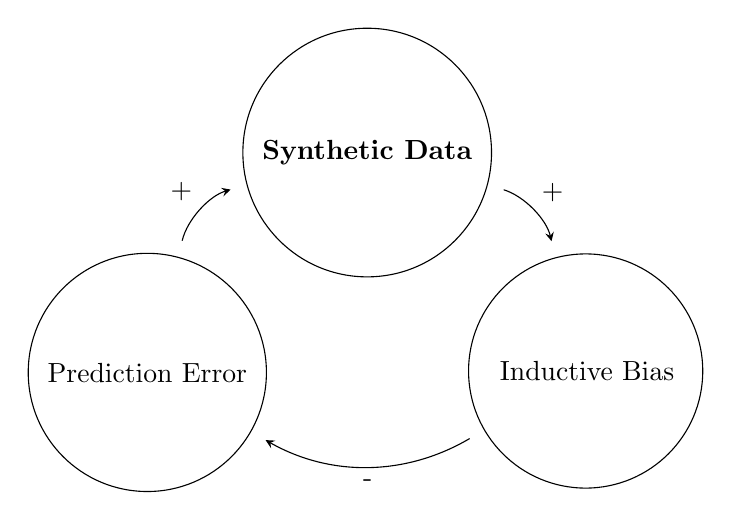
\begin{tikzpicture}[
            node distance=24pt,
            >=stealth, auto,
            every state/.style={inner sep=6pt}
        ]
        \node[state] (q14) {Prediction Error};
        \node[state] (q12) [above right=of q14] {\textbf{Synthetic Data}};
        \node[state] (q23) [below right=of q12] {\hspace{1pt} Inductive Bias \space};
            \begin{scope}[bend left]
                \path[->, shorten <= 6pt, shorten >= 6pt] 
                    (q14) edge node {+} (q12)
                    (q12) edge node {+} (q23)
                    (q23) edge node {-} (q14);
            \end{scope}
        \end{tikzpicture}
        \\~\\
        \caption{Fig. 1: Causal Loop Diagram (CLD) of synthetic data in prediction systems.}
    \end{center}
\\~\\
There are 3 components (nodes) contained within the CLD in Fig. 1, they are: Synthetic Data, Inductive Bias, and Prediction Error. These were selected because they capture the most basic theoretical components of many prediction systems with the exception of synthetic data, which was introduced as the domain of interest. The relationships (edges) between nodes were labeled with polarity ($+/-)$, a metric used later to classify the type of behavior likely to emerge as a result of the causal loop. \\

\newpage
When explaining the CLD in Fig. 1, it is best to begin at the Synthetic Data node. Take note of the polarity in relationship to the Inductive Bias node. Notice that a \textit{positive} polarity was specified, assuming that when synthetic data increases, inductive bias also increases. Moving from the Inductive Bias node to the Prediction Error node, notice that the polarity is \textit{negative}, suggesting that as inductive bias increases, prediction errors decrease (the limitation of this assumption is addressed later). Finally and perhaps most importantly, \textit{positive} polarity was specified between the Prediction Error node and the Synthetic Data node. This assumes that as prediction errors increase, sample complexity of the synthetic data increases. In other words, more synthetic data is generated when prediction errors are high.

\section*{Emergent Behavior: Balancing Loops}
    \begin{center}
        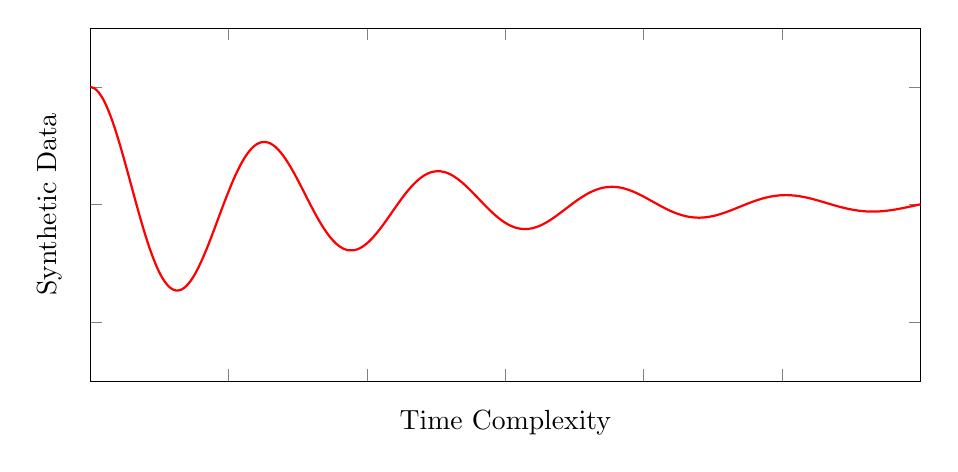
\begin{tikzpicture}
        \begin{axis}[
            xmin = 0, xmax = 30,
            ymin = -1.5, ymax = 1.5,
            width = \textwidth,
            height = 0.50\textwidth,
            xlabel near ticks, ylabel near ticks, 
            xlabel = {Time Complexity}, ylabel = {Synthetic Data},
            xticklabels={,,}, yticklabels={,,}
            ]
            \addplot[
                domain = 0:30,
                samples = 200,
                smooth,
                thick,
                red,
            ] {exp(-x/10)*( cos(deg(x)) + sin(deg(x))/10 )};
        \end{axis}
        \end{tikzpicture}
        \\~\\
        \caption{Fig. 2: Synthetic data complexity convergence over time as a $B_1$ loop.}
        \\~\\
    \end{center}

When taken together, the overall polarity of the CLD in Fig. 1 can be classified as a Balancing Loop, $B_1$. This is in contrast to a Reinforcing Loop, $R_1$, which would likely emerge in the case that the sum of polarities equal zero. In this case, the overall polarity is non-zero, which indicates that the behavior of the CLD is likely to undulated more aggressively toward the beginning of the sequence and as the time complexity increases around the causal loop, convergence is likely to occur as it approaches infinity. Again, this type of behavior is considered a $B_1$ and is exhibited in Fig. 2. Here, the sample complexity of the generated synthetic data is in response to the time complexity over the sequence of the causal loop. It is also worth mentioning that not only would the Synthetic Data node likely converge in this way, but all of the nodes would likely exhibit a similar behavior. \\

\newpage
\section*{Limitations: Linearity \& Practical Considerations}
There are two major limitations in this analysis. The first is that the polarity between corresponding nodes is assumed to be linear. The second is that the sample complexity of the synthetic data would continue in an infinite loop. \\

The first limitation arises by introducing inductive bias for reducing prediction errors. Introducing \textit{small} amounts of bias to reduce prediction errors does often work in practice. Yet, the prevailing and well accepted machine learning theory states that introducing \textit{too} much bias into prediction systems will often increase its variance, therefore increasing prediction error \cite{James2013}. In other words, the relationship between bias and variance is not often linear. However, it can be modeled as such, if it is assumed that the bias-variance trade off can be optimized to an approximate minima, where the causal loop would terminate. \\

The second limitation suggested by the diagrams is that time complexity would continue to increase beyond what would be useful for reducing prediction errors. Practically, this would not likely be the case. Generating more synthetic data would likely be halted when it was beyond what was useful in reducing prediction errors. However, it is worth mentioning that if the system were to persist with increased time complexity into infinity, we would perhaps still observe a reduction in prediction error - although a higher one than what was observed with lower time and sample complexity near the beginning of the sequence. \\

Although there are obvious limitations with many more to mention beyond the scope of this analysis, it still stands to reason that prediction errors could be useful inputs into the generation and application of synthetic data in machine learning to improve the quality of our prediction systems across a wide range of domains.

\newpage
\bibliographystyle{ieeetr}
\bibliography{ref.bib}

\end{document}